\section{Juju}\label{subsec:juju}
Juju \cite{juju_home} è un sistema open source adibito all'automazione, configurazione e deploy di infrastrutture e software per cloud ibridi e non.
% 
Sviluppato anch'esso da Canonical, ha come compito quello di aiutare gli amministratori di sistema nel deploy e semplificare la gestione software del cloud, spostando l'attenzione dalla gestione delle configurazioni delle applicazioni alla gestione delle applicazioni stesse.
% 
In questo modo i progettisti di sistemi cloud possono concentrarsi maggiormente sull'amministrazione ad alto livello delle applicazioni e degli scenari, sviluppando modelli per gestire il ridimensionamento, il coordinamento  e le dipendenze tra i vari servizi.

Aumento della scalabilità e della ridondanza, semplificazione nella gestione dell'infrastruttura e architettura del cloud e automazione nel deploy sono esempi dei vantaggi che si hanno utilizzando Juju nella creazione dei cloud.

Inoltre è possibile utilizzare Juju per gestire ambienti multi-cloud, ovvero l'utilizzo di più provider di cloud contemporaneamente, come ad esempio AWS (Amazon Web Services) per la parte computazionale e GCP (Google Cloud Platform) per lo storage.

Infine Juju può anche operare in ambienti diversi dai consueti cloud gestendoli comunque come se fossero dei veri e propri cloud, 
% ma continuando a gestire il software come se si trattasse di un cloud,
ad esempio server bare metal utilizzando MAAS o container utilizzando LXD.
% 
Questa tipologia di cloud viene anche definita \emph{substrate} \cite{juju_cloud_substrate}.



\subsection{Funzionamento: Controller e Charmed Operator}\label{subsec:juju_funzionamento}
\paragraph{Controller.} Il controller \cite{juju_controller} è il core di Juju nella gestione del cloud.
% 
Ha come compito quello di creare e gestire l'infrastruttura software del cloud ed è il responsabile dell'implementazione di tutte le modifiche richieste da parte del client Juju.
% 
Ogni controller generalmente è situato su una macchina dedicata e gestisce un singolo cloud (\cref{fig:juju_client_controllers}), quest'ultimi sono descritti attraverso i modelli.
% 
\begin{figure}[H]
    \centering
    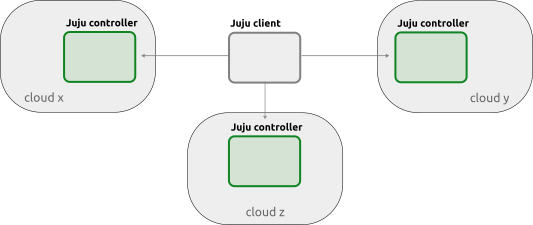
\includegraphics[width=0.8\linewidth]{tesi/files/immagini/juju/client_controllers}
    \caption{Schema del sistema Juju. Un Juju client può comunicare con più Juju controller \cite{juju_client}.}
    \label{fig:juju_client_controllers}
\end{figure}

\noindent
Un \textbf{modello} \cite{juju_model} è una collezione di applicazioni distribuite all'interno di diverse macchine.
% 
Il suo scopo è quello di consentire il raggruppamento logico di applicazioni e infrastrutture che operano e collaborano assieme per fornire un determinato servizio. 
% 
Un modello è gestito da un singolo controller, mentre un controller può gestire diversi modelli e quindi diversi set di applicazioni e macchine.

Alla creazione del controller vengono generati due modelli: il modello \emph{controller}, che conterrà solamente la macchina del controller, e il modello \emph{default}, un modello generico utilizzabile per distribuire applicazioni e macchine.
% 
\begin{figure}[H]
    \centering
    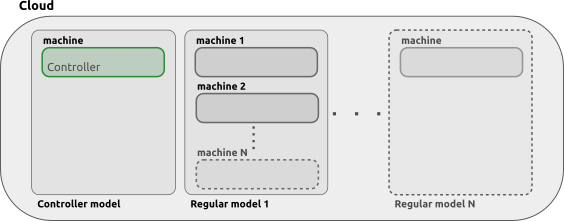
\includegraphics[width=0.8\linewidth]{tesi/files/immagini/juju/models}
    \caption{Rappresentazione del cloud in modelli. Un singolo Controller model e diversi Regular model su diverse macchine \cite{juju_model}.}
    \label{fig:juju_models}
\end{figure}
% 
\noindent 
In sintesi, un cloud è composto da un controller che gestisce vari modelli e ogni modello distribuisce applicazioni su diverse macchine (\cref{fig:juju_models}).
 

\paragraph{Charmed Operator.}
Un Charmed Operator \cite{juju_charm}, o più semplicemente \emph{Charm}, è un componente software open source che guida le fasi del ciclo di vita di una singola applicazione in tutti i suoi aspetti, come l'installazione, distribuzione, configurazione, aggiornamenti e interoperabilità con altre applicazioni.
% 
Ne gestisce inoltre le istanze, il ridimensionamento, l'ottimizzazione, il networking, semplificando la distribuzione dell'applicazione, rendendola facilmente riutilizzabile e condivisibile.

I charm sono un'espansione e una generalizzazione della nozione di operatore in Kubernetes, con la differenza che le applicazioni possono essere connesse ad altre applicazioni e possono essere distribuite non solo su cluster Kubernetes ma anche su container, VM, e macchine bare metal, sia su cloud pubblico che privato.

Esiste un'altra tipologia di charm, chiamato \emph{subordinate charmed operator}, che aumenta le funzionalità di un altro charm già esistente (in questo contesto viene denominato come \emph{principal charmed operator}).
Quando un subordinate charm viene distribuito, non viene creata una nuova istanza dell'applicazione a cui fa riferimento il principal charmed ma ne estende direttamente le funzionalità.

\bigskip
I charm sono orchestrati dal componente integrato in Juju chiamato \emph{Charmed Operator Lifecycle Manager (OLM)} \cite{juju_olm} .
% 
Questo strumento ha il compito di distribuire e mantenere aggiornate le applicazioni che i charm descrivono, provvedendo al deploy delle varie istanze delle applicazioni nelle macchine del cloud.
% 
Quando vengono scelti in fase di deploy, i charm vengono scaricati dal marketplace \emph{Charmhub} \cite{charmhub}, il luogo dove è possibile sviluppare e condividere gratuitamente i propri charm.

\subsection{Concetti chiave}\label{subsec:juju_concetti}
\paragraph{Bundle.}
% https://juju.is/docs/sdk/charm-bundles
Un bundle \cite{juju_bundle} è la rappresentazione di un modello Juju in un file in formato yaml.
% 
Al suo interno sono elencati tutti i charm, le relazioni e le configurazioni per poter effettuare il deploy del modello che rappresenta.
% 
Infatti partendo da un bundle, è possibile effettuare il deploy in maniera automatizzata di un modello, rendendolo un potente strumento indispensabile per la distribuzione di sistemi grandi e complessi in modo semplice e ripetibile.
% 
Come per i charm, è possibile trovare bundle già costruiti da altri utenti in maniera veloce e gratuita nel marketplace \emph{Charmhub} \cite{charmhub}.

\paragraph{Overlay.}
Un overlay è un'estensione del bundle.
% 
Anch'esso in formato yaml, il suo compito è quello di permettere la personalizzazione di un bundle esistente senza dover applicare direttamente le modifiche sul file, lasciando quindi inalterato l'intero bundle.
% 
In questo modo è possibile utilizzare un bundle più generico ed applicare delle personalizzazioni tramite overlay, per esempio aggiungendo charm o impostando dei vincoli personalizzati sulle macchine, o ancora modificando il numero di macchine su cui distribuire determinate applicazioni.

\paragraph{Unit.}
% https://juju.is/docs/olm/unit
Juju definisce le unit \cite{juju_unit} come le istanze di un'applicazione in esecuzione e ognuna di queste viene istanziata su macchine distinte.
% 
Durante il deploy è possibile decidere quante e su quali macchine installare le unit.
% 
Grazie alle unit è possibile dividere una singola applicazione in più istanze, garantendo in questo modo un set di repliche resiliente ai guasti e una suddivisione del carico di lavoro.
% 
Ad esempio, come mostrato in \cref{fig:juju_units} è possibile distribuire il charm mongodb su tre macchine, specificando in fase di deploy sia il numero di unit sia le macchine di destinazione.
% 
Ogni unit viene contraddistinta da un numero, preceduto dal nome dell'applicazione;
% 
ad esempio la prima unit verrà denominata "nome\_app/0".
% 
Infine, tutte le unit della stessa applicazione condividono lo stesso codice del charm, le stesse relazioni e le stesse configurazioni, ma una di esse verrà battezzata come "leader" e sarà responsabile della gestione del lifecycle dell'intera applicazione.
\begin{figure}[H]
    \centering
    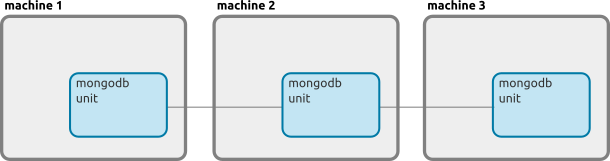
\includegraphics[width=0.8\linewidth]{tesi/files/immagini/juju/units}
    \caption{Suddivisione dell'applicazione MongoDB su tre unit \cite{juju_unit}.}
    \label{fig:juju_units}
\end{figure}


\paragraph{Relation.}
% Da Juju 3.0 si chiamano Integration
% https://juju.is/docs/olm/integration
Una relation \cite{juju_relation} (integration dalla versione 3.0 di Juju) è un protocollo di Juju che facilita lo scambio di informazioni e configurazioni tra applicazioni.
% 
Le relation di un'applicazione sono definite all'interno del charm e vengono create connettendo i vari endpoint delle applicazioni coinvolte.
% 
I vari endpoint possono essere connessi solamente se sono dello stesso tipo e se supportano la stessa interfaccia.
% 
Per esempio, come mostrato in \cref{fig:juju_relations}, il charm wordpress necessita di un database e fornisce un sito web, quindi espone rispettivamente le interfacce "mysql" e "http", alle quali è possibile (e necessario) collegare i charm mysql e apache attraverso le loro rispettive interfacce che a loro volta mettono a disposizione.

\begin{figure}[H]
    \centering
    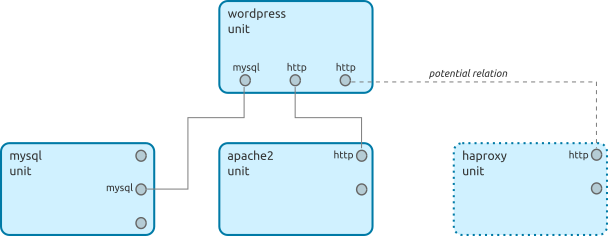
\includegraphics[width=0.9\linewidth]{tesi/files/immagini/juju/relations}
    \caption{WordPress in relation con MySQL e Apache (eventualmente anche con HAProxy) \cite{juju_relation}.}
    \label{fig:juju_relations}
\end{figure}

\noindent
Le relation possono essere facoltative o obbligatorie, a seconda delle dipendenze che charm necessita e di come è stato definito dal suo creatore.
% 

Va evidenziato che le relation non sono connessioni dirette tra i vari charm, bensì una virtualizzazione delle connessioni per consentire lo scambio di informazioni di configurazioni.
% 
Infatti è il controller Juju che ha il ruolo di mediatore per queste connessioni virtuali, gestendo il vario flusso di informazioni tra dli accessi. 

% \paragraph{Agent.}



\subsection{Installazione}\label{subsubsec:juju_install}
\paragraph{Preparazione Hardware.}
Come anticipato nella \cref{subsec:progettazione_hardware}, il  sistema cloud  progettato in questa tesi è costituito da:
\begin{itemize}
    \item Una macchina dedicata (Raspberry Pi) per il sistema MAAS (vedasi deploy nella \cref{subsubsec:maas_install}), a cui in questo capitolo verrà aggiunto il client Juju.

    \item Una macchina dedicata per il controller Juju.
    
    \item Quattro nodi sui quali verrà effettivamente installato il cloud OpenStack più un quinto per sviluppi successivi.
\end{itemize}
% 
In questo capitolo verrà trattata la sola installazione del sistema Juju, composto dal client e dal controller.

\paragraph{Preparazione software.}
L'installazione di Juju affrontata in questa sede è affiancata dallo strumento di provisioning server MAAS (\cref{subsec:maas}).
% 
Inoltre, è altre sì importante che la macchina dedicata al controller Juju sia stata aggiunta all'elenco dei nodi gestiti da MAAS (fase di elinst e commission)
% 
Pertanto, prima di procedere, è necessaria effettuare l'installazione completa del suddetto strumento e l'aggiunta dei nodi.
% 
Si vedano le \cref{subsubsec:maas_install,subsubsec:maas_conf,subsubsec:maas_add_node} per maggiori dettagli.

\bigskip
La versione di Juju che è stata installata è la 2.9.29, aggiornata poi alla 2.9.37.
% 
Il comando che verrà utilizzato in fase di installazione però installerà l'ultima versione disponibile;
% 
ciò non dovrebbe risultare problematico, ma è bene prestare attenzione che alcuni aspetti potrebbero essere differenti se si vorrà installare una versione più aggiornata.
% 
È comunque possibile, come verrà descritto poi nel \cref{lst:juju_client_install}, decidere quale versione scaricare e installare.


\paragraph{N.B.} Rispetto ad un'installazione da manuale basata sul sistema operativo Ubuntu 20.04 con architettura AMD64, quella affrontata in questa sede differisce leggermente essendo basata sul sistema operativo Raspberry Pi OS (Debian 11) con architettura ARM64.
% 
Tutte le eventuali differenze riscontrate verranno spiegate e mostrate nei dettagli.

\bigskip\noindent
 Per maggior informazioni sulle seguenti fasi di installazione, fare riferimento alla guida OpenStack \cite{juju_install_openstack} e alla documentazione Juju \cite{juju_install_doc,juju_use_maas}. %e \cite{juju_use_maas}
 % https://juju.is/docs/olm/install-juju
 % https://juju.is/docs/olm/configure-a-model
 
\subsection{Installazione e configurazione del client Juju}
Durante le fasi di installazione di Juju verranno utilizzati solamente comandi da terminale impartiti sulla macchina Raspberry Pi del sistema MAAS, diventando così anche client Juju.

\bigskip\noindent
Come prima cosa verrà installato il client Juju all'ultima versione. %alla versione 2.9.37
\begin{lstlisting}[
    language=mybash, 
    caption={Installazione del client Juju.}, 
    label={lst:juju_client_install}
]
sudo snap install ^nf^juju^nf^ --classic
\end{lstlisting}

Nel caso in cui si volesse installare un'altra versione, è possibile specificarla aggiungendo \code{-{}-channel=<version/release>}.
    Per esempio, per la versione \code{2.9.37} si va ad aggiungere \code{-{}-channel=2.9.37/stable}.

\bigskip\noindent
Fatto ciò, MAAS verrà collegato a Juju in modo tale che venga visto e gestito come se fosse un cloud.
% 
Prima verrà creato un file yaml di nome \emph{mass-cloud.yaml} contenente le seguenti configurazioni del cloud MAAS.
% 
\lstinputlisting[
    language=yaml, 
    caption={File yaml di configurazione del cloud MAAS.}, 
    label={lst:juju_maas-cloud-yaml},
]
{tesi/files/installazioni/yaml/juju/maas-cloud.yaml}
%
\begin{itemize}
    \item La dicitura \code{mass-one} indica il nome che assumerà il cloud.
    % 
    Se si vuole utilizzare un altro nome, bisogna cambiare la dicitura \code{mass-one} con il nome desiderato.

    \item In \code{type} viene indicato la tipologia del cloud; in questo caso \texttt{maas}.

    \item Con \code{auth-types} si intende il tipo di autenticazione del cloud (verrà aggiunta la chiave di autenticazione nei \cref{lst:juju_maas-creds-yaml,lst:juju_add-credential}).

    \item \code{endpoint} invece è l'URL, il punto d'accesso di MAAS inserito in fase di installazione nel \cref{lst:maas_init}.
\end{itemize}

\bigskip\noindent
A questo punto è possibile aggiungere il cloud a Juju.
% 
\begin{lstlisting}[
    language=mybash, 
    caption={Aggiunta del cloud mass-one in Juju.}, 
    label={lst:juju_add-cloud},
]
juju add-cloud --client -f maas-cloud.yaml maas-one
\end{lstlisting}
%
\begin{itemize}
    \item Con l'opzione \code{-{}-client} si va ad indicare a Juju di archiviare la definizione del cloud sulla macchina da cui si sta eseguendo il comando, ovvero il client Juju
    
    \item Con l'argomento \code{-f} viene indicato il nome del file di configurazione yaml salvato nel \cref{lst:juju_maas-cloud-yaml}
    \item Il valore \emph{mass-one} indica il nome del cloud corrispondente a quello scelto sempre nel \cref{lst:juju_maas-cloud-yaml}.
\end{itemize}
% 
Per verificare che il cloud sia stato correttamente aggiunto, si può eseguire \code{juju clouds -{}-client}; 
% 
l'output dovrebbe essere simile a quello mostrato in \cref{fig:juju_cloud_mass-one}.
% 
\begin{figure}[H]
    \centering
    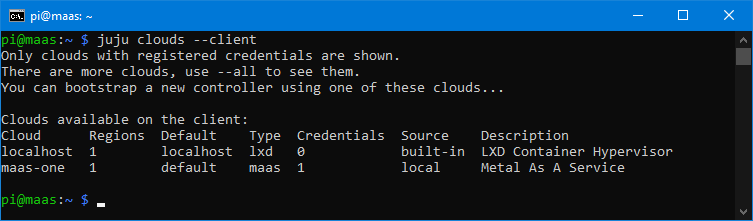
\includegraphics[width=1\linewidth]{tesi/files/immagini/juju/juju clouds}
    \caption{Elenco dei cloud presenti nel sistema Juju.}
    \label{fig:juju_cloud_mass-one}
\end{figure}

\bigskip\noindent
Una volta aggiunto il cloud MAAS, Juju ha bisogno delle credenziali per poter interagire con esso.
Verrà creato un nuovo file yaml ad hoc di nome \emph{maas-creds.yaml} avente le seguenti impostazioni.
% 
\lstinputlisting[
    language=yaml, 
    caption={File yaml contenente le credenziali del cloud MAAS.}, 
    label={lst:juju_maas-creds-yaml},
]
{tesi/files/installazioni/yaml/juju/maas-creds.yaml}
%
\begin{itemize}
    \item \code{mass-one} è il nome del cloud scelto nel \cref{lst:juju_maas-cloud-yaml}.

    \item \code{anyuser} è il nome del nuovo utente che Juju andrà ad utilizzare.

    \item Con \code{auth-type} si indica la tipologia delle credenziali da inserire.

    \item Infine in \code{maas-oauth} va indicata la chiave API che è stata salvata nel \cref{lst:maas_apikey};
    % 
    quindi sostituire \emph{admin-api-key-file} con la corrispondente chiave.
\end{itemize}

\bigskip\noindent
Ora è possibile aggiungere le credenziali a Juju.
% 
\begin{lstlisting}[
    language=mybash, 
     caption={Aggiunta delle credenziali del cloud MAAS in Juju.}, 
    label={lst:juju_add-credential},
]
juju add-credential --client -f maas-creds.yaml maas-one
\end{lstlisting}
% 
\begin{itemize}
    \item[] (Vedasi il \cref{lst:juju_add-cloud} per la spiegazione degli argomenti del comando eseguito).
\end{itemize}
% 
Anche in questo caso è possibile verificare che le credenziali siano state inserite correttamente.
% 
Per farlo, basterà eseguire \code{juju credentials -{}-client}\\\code{ -{}-show-secrets -{}-format yaml}; l'output dovrebbe essere simile a quello illustrato in \cref{fig:juju_credentials}.
% 
\begin{figure}[H]
    \centering
    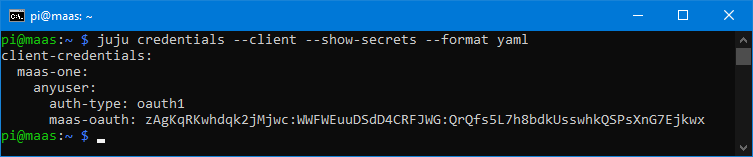
\includegraphics[width=1\linewidth]{tesi/files/immagini/juju/juju credentials}
    \caption{Elenco delle credenziali presenti nel sistema Juju.}
    \label{fig:juju_credentials}
\end{figure}

\bigskip
\subsection{Deploy del controller Juju e creazione del model}\label{sec:juju_model_create}
Arrivati a questo punto, è possibile avviare il deploy automatizzato del controller Juju.
% 
Tale richiesta verrà demandata a MAAS, il quale si occuperà dell'installazione del sistema operativo e del controller.
\begin{lstlisting}[
    language=mybash, 
    caption={Deploy del controller Juju nella macchina con tag juju.}, 
    label={lst:juju_bootstrap},
]
juju bootstrap ^c^--bootstrap-series=^c^focal --constraints "^c^tags=^c^^nf^juju^nf^ ^c^arch=^c^amd64" maas-one maas-controller
\end{lstlisting}
% \lstinputlisting[
%     language=mybash, 
%     caption={Deploy del controller Juju nella macchina con tag juju.}, 
%     label={lst:juju_bootstrap},
%     firstline=4,
%     lastline=4
% ]
% {tesi/files/installazioni/CLI/juju}
%
\begin{itemize}
    \item Con l'opzione \code{-{}-bootstrap-series} viene specificata la versione dell'immagine del sistema operativo da far installare da MAAS;
    questa verrà presa tra le immagini scaricate nel \cref{itm:image_ubuntu} nella \cref{subsubsec:maas_conf}.

    In questo caso è stata installata Ubuntu Focal, corrispondente alla versione 20.04 LTS.

    \item Con l'opzione \code{-{}-constraints} è possibile specificare in maniera precisa l'hardware a cui si sta facendo riferimento.
    % 
    In caso di più valori, questi devono essere inseriti all'interno del carattere doppio apice come mostrato nel \cref{lst:juju_bootstrap}.
    
    In questo caso è stato indicato col valore \code{tag=juju} che il comando deve essere eseguito per il nodo con il tag "juju".
    
    Inoltre, in questo specifico scenario, si è rilevato indispensabile aggiungere anche il valore \code{arch=amd64}, in quanto il comando \code{bootstrap} viene richiesto dal client Juju, situato su Raspberry Pi avente architettura ARM64 e non AMD64 come per i restanti nodi.

    Dunque in uno scenario diverso da quello presentato in questo documento, se tutte le architetture di tutte le macchine coinvolte saranno di tipo AMD64 non sarà necessario l'aggiunta del suddetto valore.

    \item \emph{mass-one} è il nome del cloud scelto nel \cref{lst:juju_maas-cloud-yaml}, mentre \emph{maas-controller} sarà il nome che assumerà il controller Juju, ovvero il controller del cloud.

\end{itemize}
% 
A comando avviato, dall'interfaccia utente web di MAAS (\cref{subsubsec:maas_conf}) dalla schermata "\emph{Machines}" sarà possibile verificare lo stato di avanzamento della fase di deploy.

Se durante la configurazione del power type dei nodi (\cref{itm:powertype} nella \cref{subsubsec:maas_add_node}) è stata scelta la modalità \emph{Manual}, la macchina del controller Juju deve essere avviata manualmente.
% 
L'intera fase di deploy richiede all'incirca una decina di minuti.
% 
A deploy terminato, la macchina del controller Juju si spegnerà e apparirà nell'elenco dei nodi sotto lo status \emph{Deployed}.

Per visualizzare l'elenco aggiornato dei controller noti al client Juju, eseguire il comando \code{juju controllers}, il cui output d'esempio viene mostrato in \cref{fig:juju_controllers}.
% 
\begin{figure}[H]
    \centering
    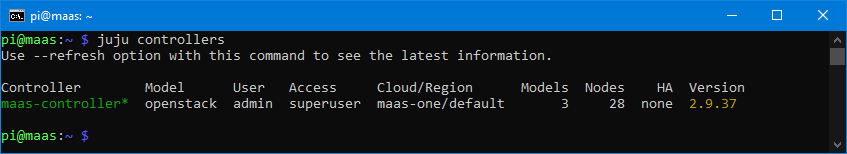
\includegraphics[width=1\linewidth]{tesi/files/immagini/juju/juju controllers}
    \caption{Elenco dei controller registrati nel client Juju.}
    \label{fig:juju_controllers}
\end{figure}

\bigskip\noindent
L'ultimo passo è quello di creare il model del cloud, al quale successivamente verranno aggiunti i vari charm che daranno corpo all'istanza effettiva del cloud.
\begin{lstlisting}[
    language=mybash, 
    caption={Creazione del model openstack per il cloud mass-one.}, 
    label={lst:juju_add-model},
]
juju add-model --config ^c^default-series=^c^jammy openstack
\end{lstlisting}
% 
\begin{itemize}
    \item Con l'opzione \code{-{}-config} è possibile specificare varie configurazioni al modello.
    Con il valore \code{default-series=} viene indicata l'immagine di default da utilizzare in fase di deploy dei nodi all'interno del cloud.
    In questo caso, l'immagine del sistema operativo è Ubuntu Jammy, corrispondente alla versione 22.04 LTS.
    
    \item Il valore \emph{openstack} sta ad indicare il nome che assumerà il model.
\end{itemize}
% 
Al termine, eseguendo il comando \code{juju status} è possibile verificare la creazione del cloud.
% 
Come mostrato in \cref{fig:juju_status1} l'output riassume il cloud appena creato.
% 
\begin{figure}[H]
    \centering
    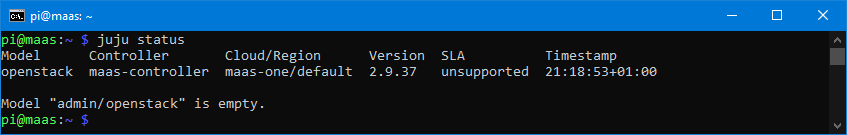
\includegraphics[width=1\linewidth]{tesi/files/immagini/juju/juju status1}
    \caption{Status del cloud vuoto mass-one.}
    \label{fig:juju_status1}
\end{figure}

\bigskip\noindent
%In \cref{sec:appendice_juju} è possibile visionare l'elenco dei comandi precedentemente descritti in un unico listato.


% accesso alla dashboard di juju
\subsection{Accesso alla dashboard}
Una volta effettuata l'installazione di Juju, è possibile accedere alla dashboard grafica attraverso il browser web.
% 
Infatti, come per MAAS, è disponibile una web app, che permette di monitorare le varie applicazioni e i vari charm all'interno del model del cloud.
% 
Eseguendo quindi il comando \code{juju dashboard} verrà mostrato L'URL per accedere all'interfaccia web, lo username e la password da utilizzare.
% 
In questo caso, l'URL dell'interfaccia web è:
% 
\begin{itemize}
    \item[]URL: \texttt{https://10.0.0.254:17070/dashboard}
\end{itemize}
% 
Mentre le credenziali da immettere sono:
% 
\begin{itemize}
    \item[]Username: \texttt{admin}

    \item[]Password: \texttt{527460c1b6b309a6bfd565924bcaacf4}
\end{itemize}

\bigskip\noindent
L'uso della dashboard è del tutto superfluo, e in questo documento non verrà ulteriormente menzionata.
% 
Tuttavia, può risultare comoda nel momento in cui si voglia andare a configurare qualche charm nello specifico;
% 
questo perché vengono mostrati direttamente le possibili configurazioni e azioni che questi possano avere, senza doverli cercare ne in documentazione ne a riga di comando.

In \cref{fig:juju_dashboard} viene mostrata la schermata d'accesso del cloud OpenStack con i charm già installati.
% 
Come è possibile vedere sono presenti sia i due model che vengono creati in automatico, ovvero il model per il \emph{controller} e il model di \emph{default}, che il model \emph{openstack}, creato nel \cref{lst:juju_add-model}.

\begin{figure}[H]
    \centering
    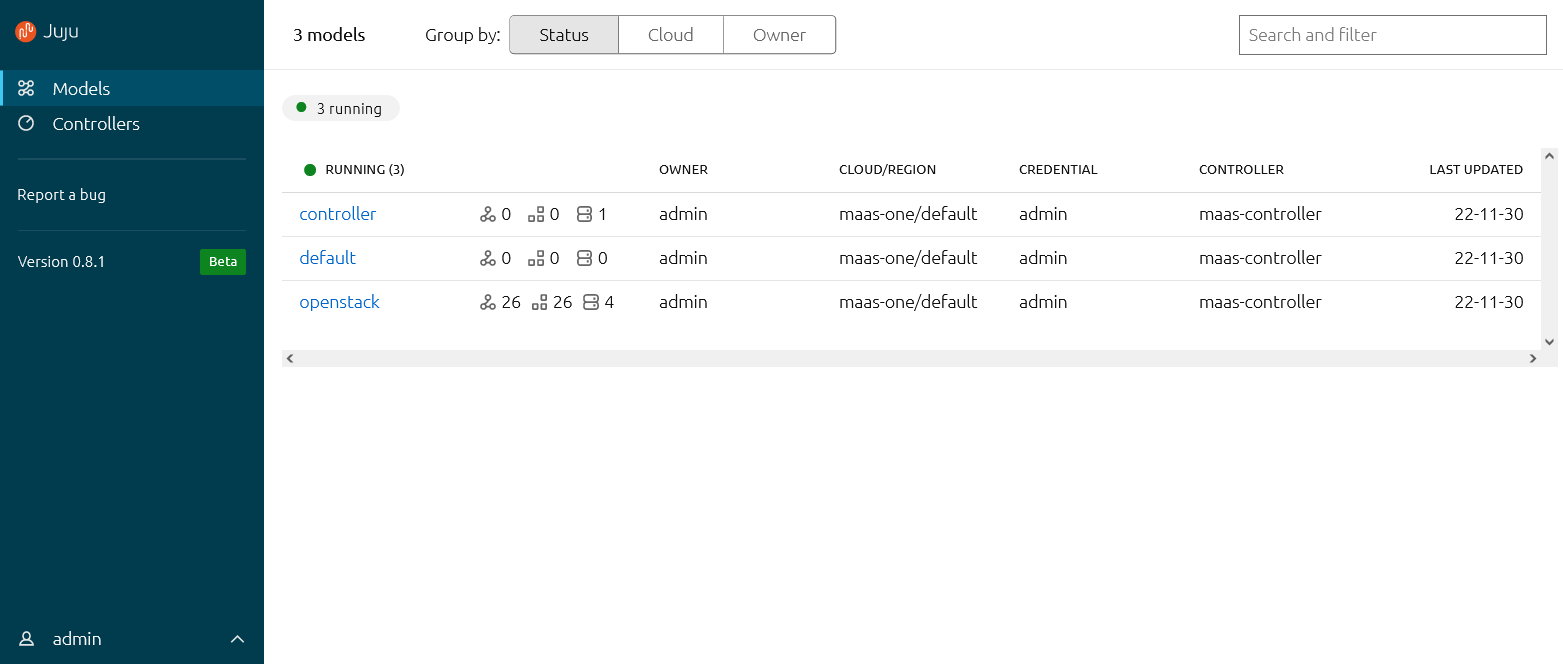
\includegraphics[width=1\linewidth]{tesi/files/immagini/juju/juju_dashboard.png}
    \caption{Esempio di schermata d'accesso della Juju dashboard.}
    \label{fig:juju_dashboard}
\end{figure}

\bigskip\noindent
Nei prossimi capitolo verrà trattata la piattaforma OpenStack, partendo da una sua descrizione e composizione, per poi passare alla completa installazione del cloud fino ad arrivare ad un suo semplice utilizzo.